%!TEX root=thesis.tex
\documentclass[thesis.tex]{subfiles}

\begin{document}

In the following three Sections I give the context and main results of my recent work. 

In \Secref{effective} I describe the development of an effective equation of motion for the orientation of a neutrally buoyant spheroid suspended in a simple shear flow, valid when inertial effects are weak but not vanishing. In short, we calculate what happens to the Jeffery orbits when the particle Reynolds number is non-zero. The results are contained in the appended Papers A-D.

The other two studies also relate to the orientational motion of non-spherical particles, and their common denominator is that they involve Jeffery's theory for ellipsoidal particles.
The first, in \Secref{experiment}, is a microfluidic experiment aiming to validate Jeffery's theory for the rotation of triaxial particles in shear flow (Paper E). The second, in \Secref{turbulence}, is a description of the rotational modes of small disks and rods in isotropic turbulence, combining data from experiments, direct numerical simulations and random flow theory (Paper F).

\chapter[Effects of inertia]{Effects of inertia on the Jeffery orbits}\label{sec:effective}

This project is a collaboration with collegues in Cherbourg and Marseille (France), and Stockholm (Sweden). J.R. Angilella (Cherbourg) and F. Candelier (Marseille) have many years of experience in dynamical systems, fluid mechanics and perturbation theory, without which this project would not have landed. T. Ros\'en and F. Lundell in Stockholm are experts in direct numerical simulation of particulate flows by the lattice Boltzmann method, by which we could validate our calculations. I also attribute the initial idea to perform stability analysis on the log-rolling motion under inertial perturbation, however vague at the time, to F. Lundell at a COST meeting in Udine, Italy. 

Paper A is a brief summary of the calculation and result in letter form, while the Papers B \& C contain all details. Paper D describes the direct numerical simulations that validate our theoretical calculation, and show in detail when the effective equations break down due to finite domain size and increasing importance of inertial effects.

\section{History of problem}

The Jeffery equations for an axisymmetric particle in simple shear flow are interesting because their solutions are degenerate, as explained in \Secref{jefferyorbits}. Their solutions form a one-parameter family of periodic orbits. No orbit is preferred over another, so that the initial condition determines the dynamics indefinitely. Jeffery was very aware of this fact, he writes \blockquote{It is obviously undesirable to leave a problem, which is physically quite determinate, in this indeterminate form.}
He further conjectures that \blockquote{this failure is due to the limitations of the theory of the slow motion of a viscous fluid.}
In other words, he believed that inertial corrections were necessary to break the degenaracy. He concludes, referring to inertial corrections, \blockquote[][...]{[...] a more complete investigation would reveal the fact that the particles do tend to adopt special orientations} 
In connection with this discussion Jeffery hypothesized that this preferred orientation would be such that the energy dissipated by viscosity is minimized: a prolate particle ends up log-rolling (long axis along the vorticity), and an oblate particle tumbles (with a diameter along vorticity.)

\citet{saffman1956} made the first attempt to include the non-linear inertial terms. It seems, although details are sparse, that he used an early form of asymptotic matching. For this he acknowledges I. Proudman, who a year later co-authored a paper \cite{proudman1957} on the inertial correction to the drag on a translating sphere, pioneering the use of asymptotic matching in viscous fluid mechanics. But Saffman did not have the proper solution to the outer ``Oseen problem'' for matching, instead he invented a plausible but ad-hoc boundary condition to match the inner expansion. With this method, applied for nearly spherical particles, he found agreement with Jeffery's minimum dissipation hypothesis.

\citet{harper1968} analyzed the rotation of two spheres rigidly constrained by an invisible rod, a so-called dumbbell. In the purely viscous regime a dumbell is equivalent to a prolate spheroid when its aspect ratio approaches infinity. They assumed that both spheres experienced lift forces (calculated by \citet{saffman1965}) independently of each other. By this method they found the opposite of Jeffery's minumum dissipation hypothesis: a slender rod ends up tumbling end-to-end in the flow-shear plane.

More recently \citet{subramanian2005,subramanian2006} re-examined the slender rod and nearly-spherical limiting cases using a reciprocal theorem \cite{kim1991,lovalenti1993}. Their method is less controversial than those employed by the earlier attemps. However, they found, like \citet{harper1968}, that for small values of the Reynolds number a slender rod tumbles end-to-end in the flow-shear plane. For larger values of the Reynolds number the tumbling orbit is destroyed and replaced by fixed points, which means that the particle stops rotating and aligns, a phenomenen observed in numerical studies \cite{ding2000} (see below). \citet{subramanian2006} found that a nearly spherical prolate particle aligns its long axis along the vorticity, and a nearly spherical oblate particle tumbles, in agreement with \citet{saffman1956}. They remark that the different types of motions for nearly spherical prolate particles, and slender prolate particles \blockquote{suggests a possible bifurcation [...] at an intermediate aspect ratio.}

Meanwhile, several groups began studies of this problem using direct numerical solution of the Navier-Stokes equations, via lattice Boltzmann simulations \cite{feng1995,ding2000,qi2003,yu2007,huang2012,rosen2014,mao2014,rosen2015a,rosen2015b}. These studies reveal a rich structure of dynamical modes for moderate to large values of the Reynolds number. Not only log-rolling or tumbling is possible, but also intermediate limit cycles and alignment with new fixed points. The studies are limited to a few particle shapes, typically $\lambda=1/4$, $\lambda=1/2$, $\lambda=2$ and $\lambda=4$. Instead they focus on the effects of increasing Reynolds numbers, confinement and particle buoyancy.

I enter this chronology sometime in 2013, after submitting a paper \cite{einarsson2014} in which we describe the effects of particle inertia alone, neglecting the fluid inertia. We were intrigued by the results of \citet{subramanian2005,subramanian2006} outlined above, and the fact that no numerical results had shown the predicted log-rolling mode for nearly spherical prolate particles. For example, \citet{qi2003} simulated both oblate ($\lambda=1/2$) and prolate ($\lambda=2$) spheroids, and found for that the oblate particle log-rolls while the prolate particle tumbles, opposite to the existing theoretical prediction. But, as \citet{subramanian2006} points out, there were several possible explanations for this discrepancy. First, the simulations were performed at moderately small Reynolds numbers, but not much smaller than unity, where a perturbation theory should be valid. Second, they were performed in a finite computational domain, whereas the theory is valid for an unbounded shear flow. Third, the particle aspect ratio $\lambda=2$ is not close to unity, whereas the theory assumed $\lambda\approx1$. The parameter ranges where the existing theory should be valid is also where the numerical simulations become computationally impractical. More precisely, small values of the Reynolds number, large distance to the boundaries, and extreme particle shape all add to the computational cost. Therefore any comparisons to existing theory were qualitative.

These facts convinced us to attempt relaxing the assumption of $\lambda\approx1$, and find the exact value of $\lambda$ for the cross-over from log-rolling to tumbling.

During my work several more numerical studies have appeared \cite{rosen2014,mao2014,rosen2015a,rosen2015b}. Despite improved methods and more raw computer power, there was still no evidence of log-rolling prolate spheroids at small values of the Reynolds number. The clearest example is in Fig.~12 of \citet{mao2014}, where they find that the dynamics of a nearly spherical particle ($\lambda=1.2$ and $\lambda=0.8$) also contradicts the theoretical prediction. Their belief is that this \blockquote{may be caused by the influence
of the higher-order effects...}, implying that the value of the Reynolds number in their simulation was out-of-range for the perturbation theory.

\section{Results}

We initially set out to calculate only the linear stability exponents of the log-rolling position. But it turned out that we could compute an explicit correction to Jeffery's equation of motion, which is more useful. Let $\ve n$ be the unit vector along the symmetry axis of the particle, and $\ma O$ and $\ma S$ the antisymmetric and symmetric parts of the shear flow gradient (see \Secref{fluidflows} for details.) Then the result is
\begin{align}
\eqnlab{ndoteffective}
  \dot {\ve n} &=  
\ma P\left[\ma O \ve n + \Lambda\ma S\ve n\right]\\
&\,+\Reys\ma P\left[b_1 (\ve n \cdot \ma S \ve n)\ma S \ve n
+ b_2 (\ve n \cdot \ma S \ve n)\ma O \ve n 
+b_3\,  \ma O \ma S \ve n 
+ b_4\,  \ma S \ma S \ve n\right]\,. \nn
\end{align}
Here the first row is the result of \citet{jeffery1922}. The projection matrix $\ma P=\ma 1 - \ve n \ve n\transpose$ removes any component of the vector field which is not tangent to the unit sphere (see also \Secref{jefferyequation}.) The scalar parameters $\Lambda$ and $b_\alpha$ depend only on the particle aspect ratio $\lambda$. The shape factor $\Lambda=(\lambda^2-1)/(\lambda^2+1)$ was computed by Jeffery. Our main accomplishment is the calculation of $b_\alpha(\lambda)$.
The result \eqnref{ndoteffective} resolves the inconsistensies between earlier theories, and between theory and numerical simulations. It also conclusively refutes Jeffery's minimum dissipation hypothesis with respect to inertia. I summarise the main conclusions in the following.

\subsection*{Linear stability analysis}

The solution to Jeffery's equation, \Eqnref{ndoteffective} with $\Reys=0$, are the degenerate periodic Jeffery orbits. In terms of the dynamical system \eqnref{ndoteffective} the phase space $S^2$ is covered by a continuous family of marginally stable periodic orbits. But just as Jeffery conjectured, an arbitrarily small amount of inertia breaks this degeneracy. The periodic orbits in phase space are replaced by a set of limit cycles and fixed points. The stable limit cycles and fixed points of \eqnref{ndoteffective} represent the preferred motions of the particle. The form of \Eqnref{ndoteffective} reveals that the vorticity direction $n_i \sim \lc_{ijk}O_{jk}$ is a fixed point, whatever the values of $\beta_\alpha(\lambda)$. This fixed point is called \emph{log-rolling}. Similarly, no trajectory of \Eqnref{ndoteffective} can cross the flow-shear plane, and therefore the phase space in that plane must contain either a limit cycle, or a set of fixed points. If it is a limit cycle, the dynamics is called \emph{tumbling}. These general features are due to the symmetries of the shear flow and the axisymmetric particle. 

\subsubsection*{First effects of inertia}
For an arbitrarily small value of $\Reys>0$ the phase space looks almost like the Jeffery orbits, but with a slow \emph{drift} between the orbits. This drift is bounded by the log-rolling and tumbling orbits, and the direction of the drift is determined by the particle shape. We determine the drift by linear stability analysis of \Eqnref{ndoteffective} to order $O(\Reys)$, and find 
\begin{itemize}
    \item $1 < \lambda < \infty$ (prolate): The particle drifts to the stable tumbling limit cycle, whatever the initial condition.
    \item $1/7.3\approx\lambda_c < \lambda < 1$ (thick oblate): The particle drifts to the stable log-rolling fixed point, whatever the initial condition.
    \item $0 < \lambda < \lambda_c$ (thin oblate): Both the log-rolling fixed point and the tumbling limit cycle are stable. Their basins of attraction are separated by one of the intermediate Jeffery orbits which have turned into an unstable limit cycle. The position of the unstable limit cycle depends on the particle shape, shown in Fig.~4 of Paper~C. 
\end{itemize}
Our result \eqnref{ndoteffective} agrees with those of \citet{subramanian2005} in the limit $\lambda\to\infty$ (up to a factor of $8\pi$). However, we find that the earlier results for nearly spherical particles \cite{saffman1956,subramanian2006} are mistaken. We have checked this in two ways. First, with F. Candelier we analysed the case of nearly spherical particles by a simultaneous perturbation around $\Reys=0$ and $\lambda=1$. We regard this complementary calculation as technically independent, because the flow solutions are expressed in spherical harmonics instead of a singularity system, and it does not use the symmetry arguments we put forward for the general case. This calculation, due mostly to F.~Candelier, is described in Paper~B. We knew that my general solution must match this special solution for nearly spherical particles exactly, as $\lambda\to1$. Once we established this equivalence we compared my solution to \citet{subramanian2005} as $\lambda\to\infty$, and found agreement up to a numerical factor of $8\pi$. We have not identified exactly where in their calculation this factor appears, but the likely culprit is in the definition of Green's functions for the Stokes flow (see App.~A.2 in Paper~C.) With these comparisons we were confident enough to submit our calculations for review and publication. The second check of our result is the direct numerical stability analysis by T. Ros\'en and F. Lundell. Our effective equation \eqnref{ndoteffective} agrees very well with the full numerical solution as $\Reys\to0$ and the computational box size becomes large. This comparison is in Paper~D (in particular Fig.~2). We conclude that our effective equation is correct. But we also see that the orientational dynamics of a non-spherical particle in shear flow is sensitive to both confinement (wall-effects), and to higher-order corrections in the shear Reynolds number.

\subsubsection*{Dynamics of oblate particles at finite values of $\Reys$}
In the previous Section I discussed the effects of inertia when $\Reys$ is arbitrarily small, but not zero. In this limit we expect the perturbative effective equation \eqnref{ndoteffective} to be valid. For larger values of $\Reys$ we cannot be certain that the dynamics of the effective equation reflects the dynamics of the exact equations. For example, the effective equation can in general not predict at which value of $\Reys$ a disk-shaped particle with $\lambda=1/12$ will cease rotating. Nevertheless, we may construct a bifurcation diagram of the effective equation in the parameter space $(\lambda, \Reys)$. We know that any bifurcation line that extends to $\Reys=0$ in the parameter space of the effective equation must \emph{connect} to a corresponding bifurcation line in the parameter space of the exact dynamics. This constrains the possible bifurcation topologies for the exact equations, and may serve as a guide for further numerical analysis.


\begin{figure}
\centering
\begin{overpic}[unit=1mm]{figs/phasediagram.pdf}
\put(70,30){\LARGE A}
\put(35,20){\LARGE B}
\put(23,33.5){\LARGE C}
\put(35,45){\LARGE D}
\put(76,64){\LARGE E}
\put(40,65){\LARGE F}
\end{overpic}
\vspace{1em}
\caption{\figlab{phasediagram} Bifurcation diagram for oblate particles ($\lambda<1$) in the effective equations \eqnref{ndoteffective}. Log-rolling is stable everywhere in this phase diagram. Regions:%
\begin{itemize}[leftmargin=2em,itemindent=0em]
    \item[A] \begin{itemize}[leftmargin=1em]
        \item[-] Tumbling orbit unstable,
        \item[-] No additional fixed points/orbits exist.
    \end{itemize}
    \item[B] \begin{itemize}[leftmargin=1em]
        \item[-] Tumbling orbit stable,
        \item[-] Limit cycle separates basins of attraction of log rolling and tumbling.
    \end{itemize}
    \item[C] \begin{itemize}[leftmargin=1em]
        \item[-] Fixed points replace tumbling orbit: one saddle, one stable node,
        \item[-] Limit cycle separates basins of attraction of log rolling and tumbling.
    \end{itemize}
    \item[D] \begin{itemize}[leftmargin=1em]
        \item[-] Fixed points replace tumbling orbit: one unstable node, one stable node,
        \item[-] Saddle point exists in interior near tumbling fixed points.
    \end{itemize}
    \item[E] \begin{itemize}[leftmargin=1em]
        \item[-] Fixed points replace tumbling orbit: one unstable node, one saddle,
        \item[-] No additional fixed points/orbits exist.
    \end{itemize}
    \item[F] \begin{itemize}[leftmargin=1em]
        \item[-] Two new fixed points are created, in total four fixed points exist in place of the tumbling orbit.
    \end{itemize}
\end{itemize} For larger values of $\Reys$ there may exist more bifurcations (not shown).}
\end{figure}

Three bifurcation lines in the parameter space of the effective equation extend to $\Reys=0$. Two of them describe the value of $\Reys$ where the tumbling orbit ceases to exist and is replaced by a pair of fixed points. Those reach $\Reys=0$ only asymptotically as $\lambda\to0$ and $\lambda\to\infty$, corresponding to infinitely thin disks or rods. The slender-body limit was described by \citet{subramanian2005}. The third bifurcation line separates the regions of stable and unstable tumbling for oblate particles, referred to in the previous Section. It connects to $\Reys=0$ at $\lambda=\lambda_c\approx1/7.3$. In Paper~D there is numerical evidence that this happens also in the exact equations. This raises the question: where does this bifurcation line go as $\Reys$ increase in the effective equation?
To answer this question I show the bifurcation diagram for oblate particles in \Figref{phasediagram}. The interesting feature of this diagram is the fate of the tumbling orbit bifurcation. It meets several other bifurcation lines in a ``critical point'' (marked by a red circle in \Figref{phasediagram}). For even larger values of $\Reys$ there may exist more bifurcations (not shown), but I expect them to be less relevant.

Numerical simulation of the exact equations reveals many different modes of rotation, depending on parameters such as particle aspect ratio, Reynolds number, confinement ratio and particle buoyancy. One may hope that the effective equation is qualitatively correct in predicting what the first bifurcation is as $\Reys$ increases. The data of \citet{rosen2015b} and Paper~D indicate that the ``critical point'', where several bifurcation lines merge, does exist also in the exact dynamics. However, the bifurcation lines seem to be sensitive to the confinement ratio in the numerical simulations and as of now we do not have enough data to confirm nor refute any claims on equivalence.

\raggedbottom\makeatletter
\afterpage{\global\let\@textbottom\relax \global\let\@texttop\relax}

\chapter[Measurements of asymmetric rods]{Measurements of asymmetric rods tumbling in microchannel flow}\seclab{experiment}
\section{Overview}
This project is a collaboration with our experimentalist collegues in Gothenburg, Sweden. Roughly the division of work is that they build and perform the experiment, and we design the specifications and perform the analysis.

The project was initiated with an intention of observing the scattering between Jeffery orbits due to thermal noise. But first we needed to observe plain Jeffery orbits, as a baseline. With hindsight that was naive, given the long list of skilled experimentalists before us who struggled with this: Sec.~II in Paper E gives a more or less exhaustive list. 

Our focus has shifted away from thermal noise, to the sensitive dependence on particle shape and initial condition. In \Secref{jefftriaxial} in Part I, I explained how Jeffery's result implies complicated dynamics for triaxial particles, even if the deviation from axisymmetry very small \cite{hinch1979,yarin1997}. We want to observe this effect in experiment.

We previously published two papers \cite{mishra2012,einarsson2013} describing our methods and some initial observations. In Paper~E we describe our most recent measurements. We are still using pressure-driven flow in a microchannel molded in PDMS plastic (\Figref{exp_setup}), but there are two main technical improvements from earlier work. First, we employ an optical trap to arrange particles for the experimental runs. This allows us to use the same particle several times, and to control its initial condition. Second, we have particles made from glass rods which have a very symmetric cross-section (see Fig.~2 in Paper~E).

\begin{figure}
\centering
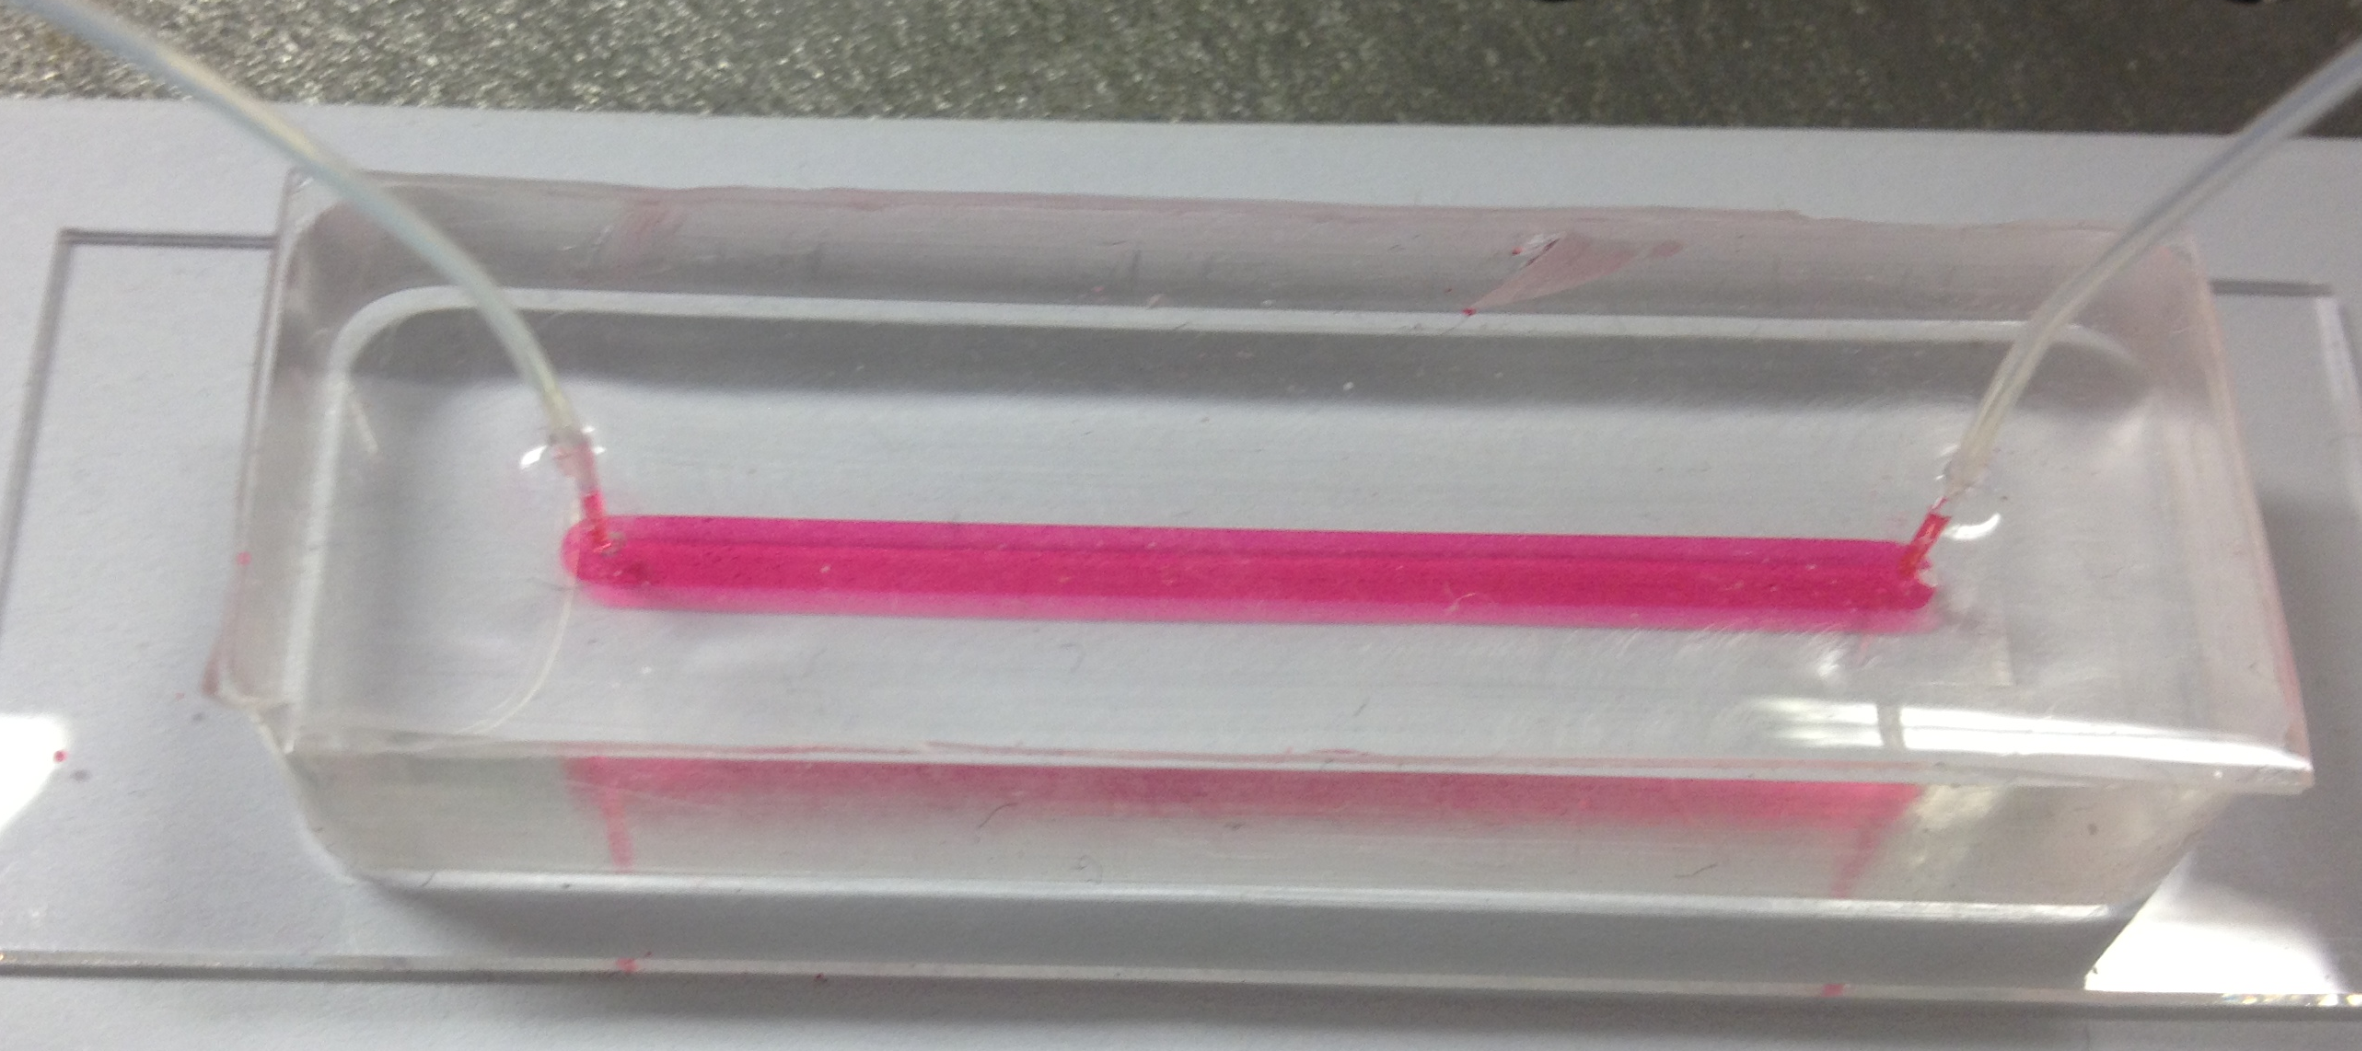
\includegraphics[width=10cm]{figs/expsetup_hires.png}%
\caption{\label{fig:exp_setup} Photograph of a microchannel of the type used in our experiment. The channel is molded in a block of PDMS plastic. In the picture the channel is filled with dye. To the left and right are inlet/outlet tubes. The channel is approximately \unit[5]{cm} long.}%
\end{figure}

In Paper~E we claim to observe both quasi-periodic and chaotic trajectories, for the same particle. Thus we confirm the predictions of \citet{hinch1979} and \citet{yarin1997}. We claim that the observed trajectories are due to the triaxial particle shape for two reasons. 

First, we reverse the pressure over the channel at the end of each particle trajectory. In the Stokes approximation the particle must then retrace its trajectory backwards, in line with the time-reversal symmetry of the Jeffery equations discussed in \Secref{jefferyequation}. If the particle trajectory does not reverse we discard the data. These reversals exclude any non-reversible effects, in particular effects of inertia or thermal noise. 

Second, with each particle we record several distinct trajectories with different initial conditions. This enables comparison with theory despite the fact that we cannot determine the particle shape accurately, because we know that all trajectories for the same particle must be consistent with the same surface-of-section of the Jeffery dynamics (see \Secref{jefftriaxial}). A complication is that we cannot measure the rotation of the rod around its long axis, that is the angle $\psi$ in the surface-of-section. However, the elliptic-island structure of the surface-of-section makes a comparison with the measured values of $n_z$ meaningful, because the dynamics are strongly influenced by the initial condition and the size of the island bounds the oscillations of $n_z$ for any trajectory.

\chapter{Rotation rates of particles in turbulence}\seclab{turbulence}
Paper~F started as the synthesis of discussions during a workshop at {\sc nordita} in Stockholm. For those I am grateful especially to E.~Variano and G.~Voth. The paper is a discussion of the rotations of axisymmetric particles in isotropic turbulence. I think the strength of this paper is it's breadth, as it contains pieces of experimental results, numerical results and analytical model calculations.

From what I remember, the discussions started because of confusion between the \emph{rotation rate} and the \emph{tumbling rate} of a particle. In this context rotation rate means magnitude of the angular velocity: $|\ve \omega|$. The tumbling rate is the rate at which the symmetry axis of the particle turns: $|\dot{\ve n}|=|\ve \omega \cross \ve n|$. The two are kinematically related, because
\begin{align}
    |\ve \omega|^2 &= |\dot{\ve n}|^2 + |\ve \omega \cdot \ve n|^2\,.
\end{align}
The difference $|\ve \omega \cdot \ve n|$ is called the \emph{spinning rate}, because it is the rate at which the particle spins around its symmetry axis.

In the paper we make two main observations. First, that the average rotation rate is roughly independent of particle shape. This is true in numerical simulations (Fig.~3 in Paper F), and in experimental measurements (Fig.~5 in Paper F.) This shape independence is unexpected, in particular because the average tumbling rate has a strong shape dependence \cite{parsa2012,gustavsson2014}. Therefore it turns out that the shape dependence of the average spinning rate almost exactly cancels the shape dependence of the average tumbling rate, as to make the total rotation rate shape independent. The reasons for this cancellation are still not known. However, in the paper we show that the average rotation rate of a particle in a random flow field is \emph{not} shape independent. This implies that the cancellation is due to the properties of the turbulent flow, and not inherent in the equations of motion.

The second main observation is on the \emph{instantaneous} rotation rates of particles. Although the average rotation rates for a thin disk and a slender rod are almost the same, their trajectories are qualitatively very different.

A key feature of turbulence is the existence of \emph{vortex tubes} \cite{she1990}. They are regions of strong vorticity, created by stretching of a large vortex into a thinner but more intensive vortex. These regions typically are long-lived, compared to the average rate of change in the flow. In these vortex tubes rod-shaped particles tend to rotate such that they keep aligned with the direction of the vorticity. The vorticity makes them spin around their own symmetry axis. But disks instead align perpendicularly to the vorticity, and the vorticity makes them tumble. But as a disk tumbles, the tumbling rate alternates between being faster and slower than vorticity, because of the flow strain. An example of this is shown in the first panel of Fig.~1 in Paper F. The rotation rate of the rod varies smoothly, and is very close to the strength of the vorticity. The rotation rate of the disk oscillates strongly, but is on average close to the strength of the vorticity.

We may partly understand these observations by a simplified picture. The effect of a rotational flow $\ve u_R= \ve \Omega \cross \ve r$ is to rotate a particle around $\ve \Omega$. The effect of a strain flow $\ve u_S=\ma S \ve r$ is to align a long axis of a particle with the strongest eigendirection of $\ma S$. The simple picture is that the same strain that stretches and intensifies a vortex to a vortex tube along $\ve \Omega$, will also align the axes of any nearby particles with $\ve \Omega$. Therefore long axes of rods, and diameters of disks tend to align with $\ve \Omega$ in these regions. With this alignment it follows that rods spin and disks tumble because of the strong vorticity.

This simple argument cannot explain why the rotation rate of the disk happens to average to the same value as that of the rod. The details of the tumbling rate depends on how the vorticity $\ve \Omega$, and the particle direction $\ve n$, are aligned relative to the eigensystem of $\ma S$. The details and implications of these alignments are important open questions. In the random-flow model these alignments are very weak, and that is the underlying reason for the shape-dependence of the average rotation rate.

\chapter{Closing words}

The past five years have been an immense learning experience for me. I was fortunate to come to Bernhard Mehlig's group around 2010. They had been working on the dynamics of particles in random flows for some time, and were increasingly interested in the theory of fluid mechanics underlying the equations of motion. I got the job as a Ph.D student, and my new job was to learn, which is a fantastic job description.

Five years later I can say that I surely learned some fluid mechanics and mathematics, but more importantly I learned about intellectual independence. I learned that independent thought requires \emph{knowing what you don't know.} It seems trivial that we should not accept, or worse, repeat, arguments that we do not understand. In my experience I am nevertheless tempted to accept an argument because I find the conclusion attractive. The most important skill I learned is to recognize and fight this temptation within myself.

During this time we also made some scientific progress, documented in Part II of this thesis and the appended papers. I end this thesis with a brief discussion of those results, and their possible future extension.

\section{Discussion of results}

Personally, the most satisfying result of my work is the description of the effect of inertia on the Jeffery orbits (Papers~A-D). First, it resolves a rather long-standing problem in theoretical fluid mechanics. The degeneracy of the Jeffery orbits is well-known, and anyone in the field immediately understands the question. Second, the result offered a couple of surprises. While the established asymptotic results for nearly spherical particles motivated us to attempt the calculation (see \Secref{effective}), they turned out to be mistaken, and there is no bifurcation of the log-rolling orbit for rod-shaped particles. On the other hand we found a non-trivial bifurcation for oblate particles of intermediate aspect ratio that I believe no-one anticipated. The original assertion that the effects of inertia breaks the degeneracy is somewhat thwarted, as the dynamics of a thin oblate particle is determined by which basin of attraction it starts in. The fact that this theoretical prediction seems to agree with new direct numerical simulations is of course very satisfying.

The experiment described in Paper~E has been a catalyst for me to dig into the dynamics of triaxial particles in shear flow. Our group has roots in research on dynamical systems, so from first sight Bernhard asked why the surfaces-of-section (\Secref{jefftriaxial}) look like those of the Hamiltonian {\lq}standard map{\rq}? Eventually, with help from S.~Östlund, we realized that the reversal symmetry we invoke in the analysis of the experiment must also imply a combined time-reversal and mirror symmetry in the equations of motion. This symmetry is not obvious in the Euler angle coordinates, because they cannot describe a mirror operation. But in the vector equations for $\ve n$ and $\ve p$ the symmetry is easily checked. In fact, I believe the symmetry should hold for any particle shape, because it is a consequence of Stokes equation.

Paper~F is different because it concerns random and turbulent flows instead of a simple shear flow. For me it was a lot of fun discussing and writing this paper, as well as our earlier paper on the same topic \cite{gustavsson2014}, because I had to learn about the statistics of turbulent flow. The main complication with angular dynamics is that the torque on a particle depends on the orientation of the particle relative to the gradients. Several groups are at work measuring, simulating and understanding these correlations between the particle orientation and the fluid gradients in turbulence. This research will contribute to our understanding of both the particle dynamics and the dynamics of the turbulent gradients, and I like to think I made a contribution towards this.

\section{Outlook}

\subsubsection{Experimental observations of angular dynamics in shear flow}
There are two obvious extensions to this work, one theoretical and one experimental.

Experimentally the next step is to measure the complete three-dimensional orientation of the particle. This is very difficult with microrods, and therefore we investigate alternative particle shapes. For example it is possible to measure the orientation of a triangular platelet using only one camera, except for some degenerate orientations which have to be determined by continuity.

The theoretical question concerns how the surface-of-section is modified for asymmetric particles. The Jeffery equation is valid for any particle with three orthogonal mirror symmetries \cite{brenner1964}. But the real particles in this experiment are not perfectly symmetric. The trajectories are sensitive to the transition from axisymmetric to triaxial, and the question is whether they are equally sensitive to breaking the mirror symmetries as well. 

\subsubsection{The effects of fluid inertia}
The reason that the calculation described in Papers~A-C is conceptually straightforward is that the Stokes flow works as the zeroth order flow field in the reciprocal theorem integral. Perturbation theory for small values of the Reynolds number is infamous, because the Stokes flow field is not a uniformly valid approximation of the flow field as $\Reys\to0$. This generally leads to a erronous or divergent result in perturbation theory. In our case this did not matter, because the erronous contribution to the volume integral of the reciprocal theorem is small. But in cases involving translational motion the volume integral diverges. We may not, for example, reproduce the Saffman lift force on a sphere translating in simple shear with just the Stokes flow field and the reciprocal theorem.

In order to solve most problems, it is necessary to construct uniformly valid flow fields to lowest order. This usually requires singular perturbation theory, of which asymptotic matching is perhaps the most common technique in fluid dynamics. Learning these methods is a necessary next step.

An interesting extension is to solve the coupled spatial and angular dynamics of a non-spherical particle in shear flow. To lowest order it makes sense to consider the rotation separately, because the Reynolds number based on the particle slip velocity is small compared to the shear Reynolds number. But at the next order of perturbation the rotation and translation are probably not decoupled. Such a calculation would be the analogue of the Saffman lift for non-spherical particles, and could make our results more relevant to inertial microfluidics.

Another effect neglected in our calculation is the effect of confinement of the particle by nearby walls. The nearby boundaries affect the nature of the inertial correction. Likely this effect can be computed similarly to the result in Paper~C, with the method of images for the multipole expansion.

Finally, in my view, a long-term goal of this research is to understand how to derive an effective equation of motion for the translational and orientational dynamics of a neutrally buoyant particle in turbulence. The Stokes drag is a good approximation for very small particles, or for finite particles if they are much heavier than the fluid. But for a neutrally buoyant particle in turbulence I expect both particle inertia and fluid inertia to contribute to an effective equation of motion.

\end{document}
